% Options for packages loaded elsewhere
\PassOptionsToPackage{unicode}{hyperref}
\PassOptionsToPackage{hyphens}{url}
\PassOptionsToPackage{dvipsnames,svgnames,x11names}{xcolor}
%
\documentclass[
  10pt,
]{article}
\usepackage{amsmath,amssymb}
\usepackage{iftex}
\ifPDFTeX
  \usepackage[T1]{fontenc}
  \usepackage[utf8]{inputenc}
  \usepackage{textcomp} % provide euro and other symbols
\else % if luatex or xetex
  \usepackage{unicode-math} % this also loads fontspec
  \defaultfontfeatures{Scale=MatchLowercase}
  \defaultfontfeatures[\rmfamily]{Ligatures=TeX,Scale=1}
\fi
\usepackage{lmodern}
\ifPDFTeX\else
  % xetex/luatex font selection
\fi
% Use upquote if available, for straight quotes in verbatim environments
\IfFileExists{upquote.sty}{\usepackage{upquote}}{}
\IfFileExists{microtype.sty}{% use microtype if available
  \usepackage[]{microtype}
  \UseMicrotypeSet[protrusion]{basicmath} % disable protrusion for tt fonts
}{}
\makeatletter
\@ifundefined{KOMAClassName}{% if non-KOMA class
  \IfFileExists{parskip.sty}{%
    \usepackage{parskip}
  }{% else
    \setlength{\parindent}{0pt}
    \setlength{\parskip}{6pt plus 2pt minus 1pt}}
}{% if KOMA class
  \KOMAoptions{parskip=half}}
\makeatother
\usepackage{xcolor}
\usepackage[left=2cm, right=2cm, top=2cm, bottom=3cm, footskip = .5cm]{geometry}
\usepackage{longtable,booktabs,array}
\usepackage{calc} % for calculating minipage widths
% Correct order of tables after \paragraph or \subparagraph
\usepackage{etoolbox}
\makeatletter
\patchcmd\longtable{\par}{\if@noskipsec\mbox{}\fi\par}{}{}
\makeatother
% Allow footnotes in longtable head/foot
\IfFileExists{footnotehyper.sty}{\usepackage{footnotehyper}}{\usepackage{footnote}}
\makesavenoteenv{longtable}
\usepackage{graphicx}
\makeatletter
\def\maxwidth{\ifdim\Gin@nat@width>\linewidth\linewidth\else\Gin@nat@width\fi}
\def\maxheight{\ifdim\Gin@nat@height>\textheight\textheight\else\Gin@nat@height\fi}
\makeatother
% Scale images if necessary, so that they will not overflow the page
% margins by default, and it is still possible to overwrite the defaults
% using explicit options in \includegraphics[width, height, ...]{}
\setkeys{Gin}{width=\maxwidth,height=\maxheight,keepaspectratio}
% Set default figure placement to htbp
\makeatletter
\def\fps@figure{htbp}
\makeatother
\setlength{\emergencystretch}{3em} % prevent overfull lines
\providecommand{\tightlist}{%
  \setlength{\itemsep}{0pt}\setlength{\parskip}{0pt}}
\setcounter{secnumdepth}{-\maxdimen} % remove section numbering
% Set up the fonts
\usepackage[urw-palatino]{mathdesign}
\usepackage[T1]{fontenc}

% Add accessibility support from http://www.richschwinn.com/accessibility
\RequirePackage{accsupp}
\RequirePackage{pdfcomment}
\newcommand{\AccTool}[2]{\BeginAccSupp{method=pdfstringdef,unicode,Alt={{#1}}}\pdftooltip{{#2}}{{#1}}\EndAccSupp{}}

% Set the language for 508
\hypersetup{
  pdftitle = {title},
  pdflang = en-US}


% Set up the headers and footers
\usepackage{graphicx}
\usepackage{fancyhdr}
\usepackage{ifthen}
%\usepackage{everypage-1x}
\usepackage{float}
%\usepackage{subfig}
%\usepackage{subcaption}

% Avoid struggling over figure and table float in Rmarkdown
\let\origfigure\figure
\let\endorigfigure\endfigure
\renewenvironment{figure}[1][2] {
    \expandafter\origfigure\expandafter[H]
} {
    \endorigfigure
}

\let\origtable\table
\let\endorigtable\endtable
\renewenvironment{table}[1][2] {
    \expandafter\origtable\expandafter[H]
} {
    \endorigtable
}

% First page has the large title and NOAA logo
\pagestyle{fancy}
\fancyhf{}
\setlength\headheight{40pt}
\fancyheadoffset[L]{0.5cm}
\cfoot{\thepage}

\fancyheadinit{%
   \ifthenelse{\value{page}=5}%
      {\fancyhead[R]{
\includegraphics[width=40pt]{images/NOAA_logo.png} \\ \textsf{\emph{March 24, 2025}}}
       \fancyhead[L]{\textsf{\LARGE State of the Ecosystem 2025: New England}}
      }%
      {\fancyhead[R]{}
       \fancyhead[L]{\textsf{\emph{State of the Ecosystem 2025: New England}}}
      }
}



\renewcommand{\headrulewidth}{0.4pt}
\renewcommand{\footrulewidth}{0pt}

% Make caption fonts a bit smaller
\usepackage[font={small}]{caption}


% Change section labels to san serif
\usepackage{sectsty}
\allsectionsfont{\normalfont\sffamily\bfseries}
\usepackage{multirow}
\usepackage{multicol}
\usepackage{colortbl}
\usepackage{hhline}
\newlength\Oldarrayrulewidth
\newlength\Oldtabcolsep
\usepackage{longtable}
\usepackage{array}
\usepackage{hyperref}
\usepackage{float}
\usepackage{wrapfig}
\ifLuaTeX
  \usepackage{selnolig}  % disable illegal ligatures
\fi
\usepackage{bookmark}
\IfFileExists{xurl.sty}{\usepackage{xurl}}{} % add URL line breaks if available
\urlstyle{same}
\hypersetup{
  colorlinks=true,
  linkcolor={Maroon},
  filecolor={Maroon},
  citecolor={Blue},
  urlcolor={blue},
  pdfcreator={LaTeX via pandoc}}

\author{}
\date{\vspace{-2.5em}}

\begin{document}

\setcounter{page}{4}
\thispagestyle{fancy}

\section{Introduction}\label{introduction}

\subsection{About This Report}\label{about-this-report}

This report is for the New England Fishery Management Council (NEFMC). The purpose of this report is to synthesize ecosystem information to allow the NEFMC to better meet fishery management objectives. The major messages of the report are synthesized on pages 1-3, with highlights of 2024 ecosystem events on page 4.
The information in this report is organized into two main sections; \hyperref[performance-relative-to-fishery-management-objectives]{performance measured against ecosystem-level management objectives} (Table \ref{tab:management-objectives}), and potential \hyperref[risks-to-meeting-fishery-management-objectives]{risks to meeting fishery management objectives} (Table \ref{tab:management-risks}: \hyperref[climate-and-ecosystem-change]{climate change} and \hyperref[other-ocean-uses-offshore-wind]{other ocean uses}). A final section highlights \hyperref[highlights]{notable 2024 ecosystem observations}.

\subsection{Report structure}\label{report-structure}

A glossary of terms\footnote{\url{https://noaa-edab.github.io/tech-doc/glossary.html}}, detailed technical methods documentation\footnote{\url{https://noaa-edab.github.io/tech-doc/}}, indicator data\footnote{\url{https://noaa-edab.github.io/ecodata/}}, and detailed indicator descriptions\footnote{\url{https://noaa-edab.github.io/catalog/index.html}} are available online. We recommend new readers first review the details of standard figure formatting (Fig. \ref{fig:docformat}a), categorization of fish and invertebrate species into feeding guilds (Table \ref{tab:species-groupings}), and definitions of ecological production units (EPUs, including the Gulf of Maine (GOM) and Georges Bank (GB); Fig. \ref{fig:docformat}b) provided at the end of the document.

The two main sections contain subsections for each management objective or potential risk. Within each subsection, we first review observed trends for indicators representing each objective or risk, including the status of the most recent data year relative to a threshold (if available) or relative to the long-term average. Second, we identify potential drivers of observed trends, and synthesize results of indicators related to those drivers to outline potential implications for management. For example, if there are multiple drivers related to an indicator trend, do indicators associated with the drivers have similar trends, and can any drivers be affected by management action(s)? We emphasize that these implications are intended to represent testable hypotheses at present, rather than ``answers,'' because the science behind these indicators and syntheses continues to develop.

\global\setlength{\Oldarrayrulewidth}{\arrayrulewidth}

\global\setlength{\Oldtabcolsep}{\tabcolsep}

\setlength{\tabcolsep}{2pt}

\renewcommand*{\arraystretch}{1}



\providecommand{\ascline}[3]{\noalign{\global\arrayrulewidth #1}\arrayrulecolor[HTML]{#2}\cline{#3}}

\begin{longtable}[c]{|p{1.77in}|p{4.09in}}

\caption{Ecosystem-scale\ fishery\ management\ objectives\ in\ New\ England}\label{tab:management-objectives}\\

\ascline{1.5pt}{666666}{1-2}

\multicolumn{1}{>{\raggedright}m{\dimexpr 1.77in+0\tabcolsep}}{\textcolor[HTML]{000000}{\fontsize{9}{9}\selectfont{Objective\ categories}}} & \multicolumn{1}{>{\raggedright}m{\dimexpr 4.09in+0\tabcolsep}}{\textcolor[HTML]{000000}{\fontsize{9}{9}\selectfont{Indicators\ reported}}} \\

\ascline{1.5pt}{666666}{1-2}\endfirsthead \caption[]{Ecosystem-scale\ fishery\ management\ objectives\ in\ New\ England}\label{tab:management-objectives}\\

\ascline{1.5pt}{666666}{1-2}

\multicolumn{1}{>{\raggedright}m{\dimexpr 1.77in+0\tabcolsep}}{\textcolor[HTML]{000000}{\fontsize{9}{9}\selectfont{Objective\ categories}}} & \multicolumn{1}{>{\raggedright}m{\dimexpr 4.09in+0\tabcolsep}}{\textcolor[HTML]{000000}{\fontsize{9}{9}\selectfont{Indicators\ reported}}} \\

\ascline{1.5pt}{666666}{1-2}\endhead



\multicolumn{2}{>{\raggedright}m{\dimexpr 5.86in+2\tabcolsep}}{\textcolor[HTML]{000000}{\fontsize{9}{9}\selectfont{\textbf{Objectives:\ Provisioning\ and\ Cultural\ Services}}}} \\





\multicolumn{1}{>{\raggedright}m{\dimexpr 1.77in+0\tabcolsep}}{\textcolor[HTML]{000000}{\fontsize{9}{9}\selectfont{Seafood\ Production}}} & \multicolumn{1}{>{\raggedright}m{\dimexpr 4.09in+0\tabcolsep}}{\textcolor[HTML]{000000}{\fontsize{9}{9}\selectfont{Landings;\ commercial\ total\ and\ by\ feeding\ guild;\ recreational\ harvest}}} \\





\multicolumn{1}{>{\raggedright}m{\dimexpr 1.77in+0\tabcolsep}}{\textcolor[HTML]{000000}{\fontsize{9}{9}\selectfont{Commercial\ Profits}}} & \multicolumn{1}{>{\raggedright}m{\dimexpr 4.09in+0\tabcolsep}}{\textcolor[HTML]{000000}{\fontsize{9}{9}\selectfont{Revenue\ decomposed\ to\ price\ and\ volume}}} \\





\multicolumn{1}{>{\raggedright}m{\dimexpr 1.77in+0\tabcolsep}}{\textcolor[HTML]{000000}{\fontsize{9}{9}\selectfont{Recreational\ Opportunities}}} & \multicolumn{1}{>{\raggedright}m{\dimexpr 4.09in+0\tabcolsep}}{\textcolor[HTML]{000000}{\fontsize{9}{9}\selectfont{Angler\ trips;\ recreational\ fleet\ diversity}}} \\





\multicolumn{1}{>{\raggedright}m{\dimexpr 1.77in+0\tabcolsep}}{\textcolor[HTML]{000000}{\fontsize{9}{9}\selectfont{Stability}}} & \multicolumn{1}{>{\raggedright}m{\dimexpr 4.09in+0\tabcolsep}}{\textcolor[HTML]{000000}{\fontsize{9}{9}\selectfont{Diversity\ indices\ (fishery\ and\ ecosystem)}}} \\





\multicolumn{1}{>{\raggedright}m{\dimexpr 1.77in+0\tabcolsep}}{\textcolor[HTML]{000000}{\fontsize{9}{9}\selectfont{Social\ \&\ Cultural}}} & \multicolumn{1}{>{\raggedright}m{\dimexpr 4.09in+0\tabcolsep}}{\textcolor[HTML]{000000}{\fontsize{9}{9}\selectfont{Community\ fishing\ engagement\ and\ social\ vulnerability\ status}}} \\





\multicolumn{1}{>{\raggedright}m{\dimexpr 1.77in+0\tabcolsep}}{\textcolor[HTML]{000000}{\fontsize{9}{9}\selectfont{Protected\ Species}}} & \multicolumn{1}{>{\raggedright}m{\dimexpr 4.09in+0\tabcolsep}}{\textcolor[HTML]{000000}{\fontsize{9}{9}\selectfont{Bycatch;\ population\ (adult\ and\ juvenile)\ numbers;\ mortalities}}} \\





\multicolumn{2}{>{\raggedright}m{\dimexpr 5.86in+2\tabcolsep}}{\textcolor[HTML]{000000}{\fontsize{9}{9}\selectfont{\textbf{Potential\ Drivers:\ Supporting\ and\ Regulating\ Services}}}} \\





\multicolumn{1}{>{\raggedright}m{\dimexpr 1.77in+0\tabcolsep}}{\textcolor[HTML]{000000}{\fontsize{9}{9}\selectfont{Management}}} & \multicolumn{1}{>{\raggedright}m{\dimexpr 4.09in+0\tabcolsep}}{\textcolor[HTML]{000000}{\fontsize{9}{9}\selectfont{Stock\ status;\ catch\ compared\ with\ catch\ limits}}} \\





\multicolumn{1}{>{\raggedright}m{\dimexpr 1.77in+0\tabcolsep}}{\textcolor[HTML]{000000}{\fontsize{9}{9}\selectfont{Biomass}}} & \multicolumn{1}{>{\raggedright}m{\dimexpr 4.09in+0\tabcolsep}}{\textcolor[HTML]{000000}{\fontsize{9}{9}\selectfont{Biomass\ or\ abundance\ by\ feeding\ guild\ from\ surveys}}} \\





\multicolumn{1}{>{\raggedright}m{\dimexpr 1.77in+0\tabcolsep}}{\textcolor[HTML]{000000}{\fontsize{9}{9}\selectfont{Environment}}} & \multicolumn{1}{>{\raggedright}m{\dimexpr 4.09in+0\tabcolsep}}{\textcolor[HTML]{000000}{\fontsize{9}{9}\selectfont{Climate\ and\ ecosystem\ risk\ indicators\ listed\ in\ Table\ 2}}} \\

\ascline{1.5pt}{666666}{1-2}



\end{longtable}



\arrayrulecolor[HTML]{000000}

\global\setlength{\arrayrulewidth}{\Oldarrayrulewidth}

\global\setlength{\tabcolsep}{\Oldtabcolsep}

\renewcommand*{\arraystretch}{1}

\newpage

\global\setlength{\Oldarrayrulewidth}{\arrayrulewidth}

\global\setlength{\Oldtabcolsep}{\tabcolsep}

\setlength{\tabcolsep}{2pt}

\renewcommand*{\arraystretch}{1}



\providecommand{\ascline}[3]{\noalign{\global\arrayrulewidth #1}\arrayrulecolor[HTML]{#2}\cline{#3}}

\begin{longtable}[c]{|p{1.00in}|p{2.20in}|p{2.80in}}

\caption{Risks\ to\ meeting\ fishery\ management\ objectives\ in\ New\ England}\label{tab:management-risks}\\

\ascline{1.5pt}{666666}{1-3}

\multicolumn{1}{>{\raggedright}m{\dimexpr 1in+0\tabcolsep}}{\textcolor[HTML]{000000}{\fontsize{9}{9}\selectfont{Risk\ categories}}} & \multicolumn{1}{>{\raggedright}m{\dimexpr 2.2in+0\tabcolsep}}{\textcolor[HTML]{000000}{\fontsize{9}{9}\selectfont{Observation\ indicators\ reported}}} & \multicolumn{1}{>{\raggedright}m{\dimexpr 2.8in+0\tabcolsep}}{\textcolor[HTML]{000000}{\fontsize{9}{9}\selectfont{Potential\ driver\ indicators\ reported}}} \\

\ascline{1.5pt}{666666}{1-3}\endfirsthead \caption[]{Risks\ to\ meeting\ fishery\ management\ objectives\ in\ New\ England}\label{tab:management-risks}\\

\ascline{1.5pt}{666666}{1-3}

\multicolumn{1}{>{\raggedright}m{\dimexpr 1in+0\tabcolsep}}{\textcolor[HTML]{000000}{\fontsize{9}{9}\selectfont{Risk\ categories}}} & \multicolumn{1}{>{\raggedright}m{\dimexpr 2.2in+0\tabcolsep}}{\textcolor[HTML]{000000}{\fontsize{9}{9}\selectfont{Observation\ indicators\ reported}}} & \multicolumn{1}{>{\raggedright}m{\dimexpr 2.8in+0\tabcolsep}}{\textcolor[HTML]{000000}{\fontsize{9}{9}\selectfont{Potential\ driver\ indicators\ reported}}} \\

\ascline{1.5pt}{666666}{1-3}\endhead



\multicolumn{3}{>{\raggedright}m{\dimexpr 6in+4\tabcolsep}}{\textcolor[HTML]{000000}{\fontsize{9}{9}\selectfont{\textbf{Climate\ and\ Ecosystem\ Risks}}}} \\





\multicolumn{1}{>{\raggedright}m{\dimexpr 1in+0\tabcolsep}}{\textcolor[HTML]{000000}{\fontsize{9}{9}\selectfont{Risks\ to\ Managing\ Spatially}}} & \multicolumn{1}{>{\raggedright}m{\dimexpr 2.2in+0\tabcolsep}}{\textcolor[HTML]{000000}{\fontsize{9}{9}\selectfont{Managed\ species\ (fish\ and\ cetacean)\ distribution\ shifts}}} & \multicolumn{1}{>{\raggedright}m{\dimexpr 2.8in+0\tabcolsep}}{\textcolor[HTML]{000000}{\fontsize{9}{9}\selectfont{Benthic\ and\ pelagic\ forage\ distribution;\ ocean\ temperature,\ changes\ in\ currents\ and\ cold\ pool}}} \\





\multicolumn{1}{>{\raggedright}m{\dimexpr 1in+0\tabcolsep}}{\textcolor[HTML]{000000}{\fontsize{9}{9}\selectfont{Risks\ to\ Managing\ Seasonally}}} & \multicolumn{1}{>{\raggedright}m{\dimexpr 2.2in+0\tabcolsep}}{\textcolor[HTML]{000000}{\fontsize{9}{9}\selectfont{Managed\ species\ spawning\ and\ migration\ timing\ changes}}} & \multicolumn{1}{>{\raggedright}m{\dimexpr 2.8in+0\tabcolsep}}{\textcolor[HTML]{000000}{\fontsize{9}{9}\selectfont{Habitat\ timing:\ Length\ of\ ocean\ summer,\ cold\ pool\ seasonal\ persistence}}} \\





\multicolumn{1}{>{\raggedright}m{\dimexpr 1in+0\tabcolsep}}{\textcolor[HTML]{000000}{\fontsize{9}{9}\selectfont{Risks\ to\ Setting\ Catch\ Limits}}} & \multicolumn{1}{>{\raggedright}m{\dimexpr 2.2in+0\tabcolsep}}{\textcolor[HTML]{000000}{\fontsize{9}{9}\selectfont{Managed\ species\ body\ condition\ and\ recruitment\ changes}}} & \multicolumn{1}{>{\raggedright}m{\dimexpr 2.8in+0\tabcolsep}}{\textcolor[HTML]{000000}{\fontsize{9}{9}\selectfont{Benthic\ and\ pelagic\ forage\ quality\ \&\ abundance:\ ocean\ temperature\ \&\ acidification\ }}} \\





\multicolumn{3}{>{\raggedright}m{\dimexpr 6in+4\tabcolsep}}{\textcolor[HTML]{000000}{\fontsize{9}{9}\selectfont{\textbf{Other\ Ocean\ Uses\ Risks}}}} \\





\multicolumn{1}{>{\raggedright}m{\dimexpr 1in+0\tabcolsep}}{\textcolor[HTML]{000000}{\fontsize{9}{9}\selectfont{Offshore\ Wind\ Risks}}} & \multicolumn{1}{>{\raggedright}m{\dimexpr 2.2in+0\tabcolsep}}{\textcolor[HTML]{000000}{\fontsize{9}{9}\selectfont{Fishery\ revenue\ and\ landings\ from\ wind\ lease\ areas\ by\ species\ and\ port}}} & \multicolumn{1}{>{\raggedright}m{\dimexpr 2.8in+0\tabcolsep}}{\textcolor[HTML]{000000}{\fontsize{9}{9}\selectfont{Wind\ development\ speed;\ Protected\ species\ presence\ and\ \ hotspots}}} \\

\ascline{1.5pt}{666666}{1-3}



\end{longtable}



\arrayrulecolor[HTML]{000000}

\global\setlength{\arrayrulewidth}{\Oldarrayrulewidth}

\global\setlength{\tabcolsep}{\Oldtabcolsep}

\renewcommand*{\arraystretch}{1}

\section{Performance Relative to Fishery Management Objectives}\label{performance-relative-to-fishery-management-objectives}

In this section, we examine indicators related to broad, ecosystem-level fishery management objectives. We also provide hypotheses on the implications of these trends---why we are seeing them, what's driving them, and potential or observed regime shifts or changes in ecosystem structure. Identifying multiple drivers, regime shifts, and potential changes to ecosystem structure, as well as identifying the most vulnerable resources, can help managers determine whether anything needs to be done differently to meet objectives and how to prioritize upcoming issues/risks.

\subsection{Seafood Production}\label{seafood-production}

\subsubsection{Indicators: Landings; commercial and recreational}\label{indicators-landings-commercial-and-recreational}

This year, we present updated indicators for total \href{https://noaa-edab.github.io/catalog/comdat.html}{commercial landings}, U.S. seafood landings (includes seafood, bait, and industrial landings), and Council-managed U.S. seafood landings through 2023. There are long-term declines in all New England landings time series except for total commercial landings on GB (Fig. \ref{fig:total-landings}). There exist long-term declines in commercial seafood landings and NEFMC managed seafood landings for both the GOM and GB, but over the last decade there is no trend in managed seafood landings in the GOM.

\begin{figure}

{\centering 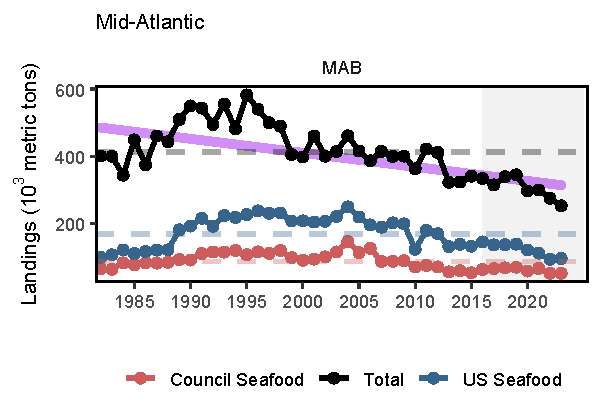
\includegraphics{C:/Users/abigail.tyrell/Documents/code/READ-EDAB-SOE_reports/output/parent_report_newengland_files/figure-latex/total-landings-1} 

}

\caption{Total commercial landings (black), total U.S. seafood landings (blue), and New England managed U.S. seafood landings (red) for Georges Bank (GB) and the Gulf of Maine (GOM).}\label{fig:total-landings}
\end{figure}

\end{document}
